% Options for packages loaded elsewhere
\PassOptionsToPackage{unicode}{hyperref}
\PassOptionsToPackage{hyphens}{url}
%
\documentclass[
  ignorenonframetext,
]{beamer}
\usepackage{pgfpages}
\setbeamertemplate{caption}[numbered]
\setbeamertemplate{caption label separator}{: }
\setbeamercolor{caption name}{fg=normal text.fg}
\beamertemplatenavigationsymbolsempty
% Prevent slide breaks in the middle of a paragraph
\widowpenalties 1 10000
\raggedbottom
\setbeamertemplate{part page}{
  \centering
  \begin{beamercolorbox}[sep=16pt,center]{part title}
    \usebeamerfont{part title}\insertpart\par
  \end{beamercolorbox}
}
\setbeamertemplate{section page}{
  \centering
  \begin{beamercolorbox}[sep=12pt,center]{part title}
    \usebeamerfont{section title}\insertsection\par
  \end{beamercolorbox}
}
\setbeamertemplate{subsection page}{
  \centering
  \begin{beamercolorbox}[sep=8pt,center]{part title}
    \usebeamerfont{subsection title}\insertsubsection\par
  \end{beamercolorbox}
}
\AtBeginPart{
  \frame{\partpage}
}
\AtBeginSection{
  \ifbibliography
  \else
    \frame{\sectionpage}
  \fi
}
\AtBeginSubsection{
  \frame{\subsectionpage}
}
\usepackage{amsmath,amssymb}
\usepackage{lmodern}
\usepackage{ifxetex,ifluatex}
\ifnum 0\ifxetex 1\fi\ifluatex 1\fi=0 % if pdftex
  \usepackage[T1]{fontenc}
  \usepackage[utf8]{inputenc}
  \usepackage{textcomp} % provide euro and other symbols
\else % if luatex or xetex
  \usepackage{unicode-math}
  \defaultfontfeatures{Scale=MatchLowercase}
  \defaultfontfeatures[\rmfamily]{Ligatures=TeX,Scale=1}
\fi
\usetheme[]{BIGSSS}
\usefonttheme{professionalfonts}
% Use upquote if available, for straight quotes in verbatim environments
\IfFileExists{upquote.sty}{\usepackage{upquote}}{}
\IfFileExists{microtype.sty}{% use microtype if available
  \usepackage[]{microtype}
  \UseMicrotypeSet[protrusion]{basicmath} % disable protrusion for tt fonts
}{}
\makeatletter
\@ifundefined{KOMAClassName}{% if non-KOMA class
  \IfFileExists{parskip.sty}{%
    \usepackage{parskip}
  }{% else
    \setlength{\parindent}{0pt}
    \setlength{\parskip}{6pt plus 2pt minus 1pt}}
}{% if KOMA class
  \KOMAoptions{parskip=half}}
\makeatother
\usepackage{xcolor}
\IfFileExists{xurl.sty}{\usepackage{xurl}}{} % add URL line breaks if available
\IfFileExists{bookmark.sty}{\usepackage{bookmark}}{\usepackage{hyperref}}
\hypersetup{
  pdftitle={The Political Economy of Higher Education: Preferences, Inequality, and Policy Change},
  pdfauthor={Timm Fulge},
  hidelinks,
  pdfcreator={LaTeX via pandoc}}
\urlstyle{same} % disable monospaced font for URLs
\newif\ifbibliography
\usepackage{color}
\usepackage{fancyvrb}
\newcommand{\VerbBar}{|}
\newcommand{\VERB}{\Verb[commandchars=\\\{\}]}
\DefineVerbatimEnvironment{Highlighting}{Verbatim}{commandchars=\\\{\}}
% Add ',fontsize=\small' for more characters per line
\usepackage{framed}
\definecolor{shadecolor}{RGB}{248,248,248}
\newenvironment{Shaded}{\begin{snugshade}}{\end{snugshade}}
\newcommand{\AlertTok}[1]{\textcolor[rgb]{0.94,0.16,0.16}{#1}}
\newcommand{\AnnotationTok}[1]{\textcolor[rgb]{0.56,0.35,0.01}{\textbf{\textit{#1}}}}
\newcommand{\AttributeTok}[1]{\textcolor[rgb]{0.77,0.63,0.00}{#1}}
\newcommand{\BaseNTok}[1]{\textcolor[rgb]{0.00,0.00,0.81}{#1}}
\newcommand{\BuiltInTok}[1]{#1}
\newcommand{\CharTok}[1]{\textcolor[rgb]{0.31,0.60,0.02}{#1}}
\newcommand{\CommentTok}[1]{\textcolor[rgb]{0.56,0.35,0.01}{\textit{#1}}}
\newcommand{\CommentVarTok}[1]{\textcolor[rgb]{0.56,0.35,0.01}{\textbf{\textit{#1}}}}
\newcommand{\ConstantTok}[1]{\textcolor[rgb]{0.00,0.00,0.00}{#1}}
\newcommand{\ControlFlowTok}[1]{\textcolor[rgb]{0.13,0.29,0.53}{\textbf{#1}}}
\newcommand{\DataTypeTok}[1]{\textcolor[rgb]{0.13,0.29,0.53}{#1}}
\newcommand{\DecValTok}[1]{\textcolor[rgb]{0.00,0.00,0.81}{#1}}
\newcommand{\DocumentationTok}[1]{\textcolor[rgb]{0.56,0.35,0.01}{\textbf{\textit{#1}}}}
\newcommand{\ErrorTok}[1]{\textcolor[rgb]{0.64,0.00,0.00}{\textbf{#1}}}
\newcommand{\ExtensionTok}[1]{#1}
\newcommand{\FloatTok}[1]{\textcolor[rgb]{0.00,0.00,0.81}{#1}}
\newcommand{\FunctionTok}[1]{\textcolor[rgb]{0.00,0.00,0.00}{#1}}
\newcommand{\ImportTok}[1]{#1}
\newcommand{\InformationTok}[1]{\textcolor[rgb]{0.56,0.35,0.01}{\textbf{\textit{#1}}}}
\newcommand{\KeywordTok}[1]{\textcolor[rgb]{0.13,0.29,0.53}{\textbf{#1}}}
\newcommand{\NormalTok}[1]{#1}
\newcommand{\OperatorTok}[1]{\textcolor[rgb]{0.81,0.36,0.00}{\textbf{#1}}}
\newcommand{\OtherTok}[1]{\textcolor[rgb]{0.56,0.35,0.01}{#1}}
\newcommand{\PreprocessorTok}[1]{\textcolor[rgb]{0.56,0.35,0.01}{\textit{#1}}}
\newcommand{\RegionMarkerTok}[1]{#1}
\newcommand{\SpecialCharTok}[1]{\textcolor[rgb]{0.00,0.00,0.00}{#1}}
\newcommand{\SpecialStringTok}[1]{\textcolor[rgb]{0.31,0.60,0.02}{#1}}
\newcommand{\StringTok}[1]{\textcolor[rgb]{0.31,0.60,0.02}{#1}}
\newcommand{\VariableTok}[1]{\textcolor[rgb]{0.00,0.00,0.00}{#1}}
\newcommand{\VerbatimStringTok}[1]{\textcolor[rgb]{0.31,0.60,0.02}{#1}}
\newcommand{\WarningTok}[1]{\textcolor[rgb]{0.56,0.35,0.01}{\textbf{\textit{#1}}}}
\usepackage{graphicx}
\makeatletter
\def\maxwidth{\ifdim\Gin@nat@width>\linewidth\linewidth\else\Gin@nat@width\fi}
\def\maxheight{\ifdim\Gin@nat@height>\textheight\textheight\else\Gin@nat@height\fi}
\makeatother
% Scale images if necessary, so that they will not overflow the page
% margins by default, and it is still possible to overwrite the defaults
% using explicit options in \includegraphics[width, height, ...]{}
\setkeys{Gin}{width=\maxwidth,height=\maxheight,keepaspectratio}
% Set default figure placement to htbp
\makeatletter
\def\fps@figure{htbp}
\makeatother
\setlength{\emergencystretch}{3em} % prevent overfull lines
\providecommand{\tightlist}{%
  \setlength{\itemsep}{0pt}\setlength{\parskip}{0pt}}
\setcounter{secnumdepth}{-\maxdimen} % remove section numbering
\AtBeginEnvironment{CSLReferences}{\tiny}
\ifluatex
  \usepackage{selnolig}  % disable illegal ligatures
\fi
\newlength{\cslhangindent}
\setlength{\cslhangindent}{1.5em}
\newlength{\csllabelwidth}
\setlength{\csllabelwidth}{3em}
\newenvironment{CSLReferences}[2] % #1 hanging-ident, #2 entry spacing
 {% don't indent paragraphs
  \setlength{\parindent}{0pt}
  % turn on hanging indent if param 1 is 1
  \ifodd #1 \everypar{\setlength{\hangindent}{\cslhangindent}}\ignorespaces\fi
  % set entry spacing
  \ifnum #2 > 0
  \setlength{\parskip}{#2\baselineskip}
  \fi
 }%
 {}
\usepackage{calc}
\newcommand{\CSLBlock}[1]{#1\hfill\break}
\newcommand{\CSLLeftMargin}[1]{\parbox[t]{\csllabelwidth}{#1}}
\newcommand{\CSLRightInline}[1]{\parbox[t]{\linewidth - \csllabelwidth}{#1}\break}
\newcommand{\CSLIndent}[1]{\hspace{\cslhangindent}#1}

\title{The Political Economy of Higher Education: Preferences,
Inequality, and Policy Change}
\subtitle{Dissertationskolloquium}
\author{Timm Fulge}
\date{13. Mai 2022}

\begin{document}
\frame{\titlepage}

\begin{frame}{Einstieg}
\protect\hypertarget{einstieg}{}
\includegraphics{Figures/FiguresEnrolment_over_time_new-1.pdf} \pause

\begin{itemize}
\item{Genereller Trend zur Expansion}
\item{Hochschulbildung: Bemerkenswerte Varianz zwischen einzelnen Ländern (nicht nur in Bezug auf Enrolment)}
\end{itemize}
\end{frame}

\begin{frame}{Einstieg}
\protect\hypertarget{einstieg-1}{}
Higher Education is special!

\pause

\begin{alertblock}{Leitfragen}
\begin{itemize}[<+->]
\item{Wie können Hochschulsysteme möglichst ganzheitlich konzeptualisiert werden?}
\item{Welche Varianz zeigt sich zwischen Ländern sowie über die Zeit?}
\item{Welche (re)distributiven Implikationen haben unterschiedliche Designs von Hochschulsystemen?}
\item{Wie können Unterschiede erklärt werden?}
\begin{itemize}
\item{Sozio-ökonomischer Problemdruck}
\item{Pfadabhängigkeiten}
\item{Parteipolitik}
\end{itemize}
\end{itemize}
\end{alertblock}
\end{frame}

\begin{frame}{Einstieg}
\protect\hypertarget{einstieg-2}{}
\textbf{Kumulative Dissertation}, auf Englisch verfasst und bestehend
Introduction und drei Einzelarbeiten in alleiniger Autorenschaft:

\begin{itemize}
\item{\textit{The Trilemma of Higher Education and Equality of Opportunity: Social Background, Access to Higher Education and the Moderating Impact of Enrolment and Public Subsidization}}
\item{\textit{Explaining Institutional Change in UK Higher Education: Towards A Partisan Theory?}}
\item{\textit{The Role of Parties in the Distributive Politics of Higher Education}}
\end{itemize}
\end{frame}

\begin{frame}{Stand der Forschung}
\protect\hypertarget{stand-der-forschung}{}
\begin{figure}
\centering
\includegraphics{Figures/Intro/EvolutionOfTheField.drawio.pdf}
\caption{Evolution der Literatur zum Forschungsgegenstand}
\end{figure}
\end{frame}

\begin{frame}{Konzeptioneller Rahmen}
\protect\hypertarget{konzeptioneller-rahmen}{}
\begin{figure}
\centering
\includegraphics{Figures/Intro/polecon_final.drawio.pdf}
\caption{Modell der politischen Ökonomie der Hochschulbildung}
\end{figure}
\end{frame}

\begin{frame}{Paper \#1: \emph{The Trilemma of Higher Education and
Equality of Opportunity} (Forschungsdesign)}
\protect\hypertarget{paper-1-the-trilemma-of-higher-education-and-equality-of-opportunity-forschungsdesign}{}
\begin{block}{Forschungsfrage}
\scriptsize
Wie strukturiert das institutionelle Design des Hochschulsystems den Zugang zu universitärer Bildung? Mindert oder verstärkt es Effekte sozialer Herkunft?
\end{block}

\pause

\begin{exampleblock}{Theorie}
\begin{itemize}
\scriptsize
\item{Ungleichheitsbezogene Bildungsforschung: Soziale Herkunft (hier = elterlicher Bildungsstand) sagt systematisch Erfolg im Bildungssystem voraus}
\begin{itemize}
\scriptsize
\item{Kosten-Nutzen-Kalkulation: $P_{HE} = (p * U) - C_{HE}$}
\end{itemize}
\item{Politische Ökonomie der Hochschulbildung: Studierendenzahl (\textit{Enrolment}) und Level öffentlicher Bezuschussung (\textit{Public Subsidization}) könnte Kosten-Nutzen-Kalkulation beeinflussen}
\end{itemize}
\end{exampleblock}

\pause

\begin{alertblock}{Daten \& Methode}
\begin{itemize}
\scriptsize
\item{Zentrale Variablen: \textit{Student} (AV); \textit{Parental Education}, \textit{Enrolment}, \textit{Public Subsidization} (UVs)}
\item{Daten: Gepoolte Wellen des European Social Survey (2002-2010), Makrodaten vom UNESCO Institute for Statistics (22 Länder, 16.278 Beobachtungen)}
\item{Methode: Hierarchische logistische Regression mit Random Intercepts + Slopes}
\end{itemize}
\end{alertblock}
\end{frame}

\begin{frame}{Paper \#1: \emph{The Trilemma of Higher Education and
Equality of Opportunity} (Ergebnisse)}
\protect\hypertarget{paper-1-the-trilemma-of-higher-education-and-equality-of-opportunity-ergebnisse}{}
\textbf{H1:} Je niedriger das elterliche Bildungsniveau, desto geringer
die Wahrscheinlichkeit, ein Studium aufzunehmen \scriptsize 
\(logit\{Pr(Student_{ij} = 1|,x_{ij}|,\zeta_{j})\} = \beta_{1} + \beta_{2}Parental\:Education_{ij} + \cdots + \zeta_{j} + \epsilon_{ij}\)

\begin{figure}
\includegraphics[width=55.56in,height=5cm]{Figures/01_Inequality/Figure 4} \caption{Geschätzte Randmittel, Fixed Effect von elterlicher Bildung auf Studiumswahrscheinlichkeit}\label{fig:unnamed-chunk-4}
\end{figure}
\end{frame}

\begin{frame}{Paper \#1: \emph{The Trilemma of Higher Education and
Equality of Opportunity} (Ergebnisse)}
\protect\hypertarget{paper-1-the-trilemma-of-higher-education-and-equality-of-opportunity-ergebnisse-1}{}
\textbf{H2:} Die Effektstärke der elterlichen Bildung auf die
Studiumswahrscheinlichkeit variiert zwischen den Ländern \scriptsize 
\(logit\{Pr(Student_{ij} = 1|,x_{ij}|,\zeta_{j})\} = \beta_{1} + \beta_{2}x_{2ij} + \cdots + \zeta_{j}Parental\:Education_{ij} + \epsilon_{ij}\)

\begin{figure}
\includegraphics[width=55.56in,height=5cm]{Figures/01_Inequality/Figure 3} \caption{Effekt elterlicher Bildung auf Studiumswahrscheinlichkeit, nach Ländern}\label{fig:unnamed-chunk-5}
\end{figure}
\end{frame}

\begin{frame}{Paper \#1: \emph{The Trilemma of Higher Education and
Equality of Opportunity} (Ergebnisse)}
\protect\hypertarget{paper-1-the-trilemma-of-higher-education-and-equality-of-opportunity-ergebnisse-2}{}
\textbf{H3:} Die Effektstärke der elterlichen Bildung auf die
Studiumswahrscheinlichkeit wird (auch) vom institutionellen Design des
Hochschulsystems (\emph{Enrolment}, \emph{Public Subsidization})
beeinflusst \scriptsize 
\(logit\{Pr(Student_{ij} = 1|,x_{ij}|,\zeta_{j})\} = \beta_{1} + \beta_{2}Parental\:Education_{ij} *\beta_{3}Enrolment\: /\: Public\:Subsidization_{j} + \cdots + \zeta_{j} + \epsilon_{i}\)

\begin{figure}
\includegraphics[width=14.25in,height=5cm]{Figures/01_Inequality/RegTablet} \end{figure}
\end{frame}

\begin{frame}{Paper \#1: \emph{The Trilemma of Higher Education and
Equality of Opportunity} (Ergebnisse)}
\protect\hypertarget{paper-1-the-trilemma-of-higher-education-and-equality-of-opportunity-ergebnisse-3}{}
\textbf{H3:} Die Effektstärke der elterlichen Bildung auf die
Studiumswahrscheinlichkeit wird (auch) vom institutionellen Design des
Hochschulsystems (\emph{Enrolment}, \emph{Public Subsidization})
beeinflusst \scriptsize 
\(logit\{Pr(Student_{ij} = 1|,x_{ij}|,\zeta_{j})\} = \beta_{1} + \beta_{2}Parental\:Education_{ij} *\beta_{3}Enrolment\: /\: Public\:Subsidization_{j} + \cdots + \zeta_{j} + \epsilon_{i}\)

\begin{figure}
\includegraphics[width=55.56in,height=5cm]{Figures/01_Inequality/Figure5} \caption{Cross-Level Interaktionseffekt von elterlicher Bildung und öffentlicher Bezuschussung auf Studiumswahrscheinlichkeit}\label{fig:unnamed-chunk-7}
\end{figure}
\end{frame}

\begin{frame}{Paper \#1: \emph{The Trilemma of Higher Education and
Equality of Opportunity} (Zusammenfassung)}
\protect\hypertarget{paper-1-the-trilemma-of-higher-education-and-equality-of-opportunity-zusammenfassung}{}
\begin{itemize}
\tightlist
\item
  Länderübergreifend starker Einfluss von sozialem Hintergrund auf
  Studiumswahrscheinlichkeit \pause
\item
  Effektstärke variiert erheblich zwischen den Ländern \pause
\item
  Teil der Varianz zwischen den Ländern kann mit dem Level öffentlicher
  Bezuschussung erklärt werden: Je generöser studentischer Subventionen
  sind, desto geringer fällt der Einfluss des sozialen Hintergrunds auf
  die Studiumswahrscheinlichkeit aus. Kein Effekt der Studierendenquote.
  \pause
\item
  Empirische Implikation: Trend zur Expansion des Hochschulsystems auf
  Kosten der Generösität der Subventionen könnte sich negativ auf
  sozialen Gradient auswirken

  \begin{figure}
  \includegraphics[width=55.56in,height=5cm]{Figures/01_Inequality/Figure2} \caption{Entwicklung der Hochschulsysteme, Veränderung 2002-2010}\label{fig:unnamed-chunk-8}
  \end{figure}
\end{itemize}
\end{frame}

\begin{frame}{Paper \#2: \emph{Explaining Institutional Change in UK
Higher Education: Towards A Partisan Theory?} (Forschungsdesign)}
\protect\hypertarget{paper-2-explaining-institutional-change-in-uk-higher-education-towards-a-partisan-theory-forschungsdesign}{}
\begin{block}{Forschungsfragen}
\scriptsize
\begin{itemize}
\item{Wie kann das institutionelle Design von Hochschulsystemen beschrieben und über die Zeit nachgezeichnet werden?}
\item{Mit welchen Hemmnissen und Zielkonflikten ist die Politik bei Reformbemühungen konfrontiert?}
\item{Können generalisierbare parteipolitische Präferenzen zum Design von Hochschulsystemen identifiziert werden?}
\end{itemize}
\end{block}

\pause

\begin{exampleblock}{Theorie}
\begin{itemize}
\scriptsize
\item{Theoriebildender Ansatz}
\item{Analytischer Rahmen: Historischer Institutionalismus nach Kathleen Thelen (Thelen 2004, Streeck \& Thelen 2005, Mahoney \& Thelen 2010)}
\end{itemize}
\end{exampleblock}

\pause

\begin{alertblock}{Daten \& Methode}
\begin{itemize}
\scriptsize
\item{Daten: Primär- und Sekundärliteratur}
\item{Methode: Dichte Beschreibung / Process Tracing}
\item{Fallauswahl: Diverse case-selection strategy nach Gerring (2007), vier Reformperioden zwischen 1963-2015}
\end{itemize}
\end{alertblock}
\end{frame}

\begin{frame}{Paper \#2: \emph{Explaining Institutional Change in UK
Higher Education: Towards A Partisan Theory?} (Ergebnisse)}
\protect\hypertarget{paper-2-explaining-institutional-change-in-uk-higher-education-towards-a-partisan-theory-ergebnisse}{}
\textbf{Vier Perioden von Reformaktivität}

\begin{itemize}
\item{Nachkriegskonsens (1963-1979)}
\begin{itemize}
\item{Moderate, gut finanzierte Expansion des Hochschulsektors}
\item{Großzügige Subventionen für Studierende, aber ausgeprägte soziale Ungleichheiten beim Hochschulzugang}
\item{Hohes Maß an Qualität / Pro-Kopf-Finanzierung}
\end{itemize}
\item{Kürzungspolitik unter Tory-Regierungen (1979-1997)}
\item{Wandel unter Labour (1997-2010)}
\item{Tory-LibDem Koalition, 2010-2015}
\end{itemize}
\end{frame}

\begin{frame}{Paper \#2: \emph{Explaining Institutional Change in UK
Higher Education: Towards A Partisan Theory?} (Ergebnisse)}
\protect\hypertarget{paper-2-explaining-institutional-change-in-uk-higher-education-towards-a-partisan-theory-ergebnisse-1}{}
\textbf{Vier Perioden von Reformaktivität}

\begin{itemize}
\item{Nachkriegskonsens (1963-1979)}
\item{Kürzungspolitik unter Tory-Regierungen (1979-1997)}
\begin{itemize}
\item{Massive Kürzungen der öffentlichen Mittel für Universitäten}
\item{Zunächst Stagnation der Studierendenquote, später massive Expansion}
\item{$\rightarrow$ Halbierung der Pro-Kopf-Finanzierung}
\item{Reduzierung der Generösität von Stipendien für Studierende, Einführung von Studienkrediten}
\item{Element der Stratifikation innterhalb des Hochschulsektors, Schutz der Eliteinstitutionen}
\end{itemize}
\item{Wandel unter Labour (1997-2010)}
\item{Tory-LibDem Koalition, 2010-2015}
\end{itemize}
\end{frame}

\begin{frame}{Paper \#2: \emph{Explaining Institutional Change in UK
Higher Education: Towards A Partisan Theory?} (Ergebnisse)}
\protect\hypertarget{paper-2-explaining-institutional-change-in-uk-higher-education-towards-a-partisan-theory-ergebnisse-2}{}
\textbf{Vier Perioden von Reformaktivität}

\begin{itemize}
\item{Nachkriegskonsens (1963-1979)}
\item{{Kürzungspolitik unter Tory-Regierungen (1979-1997)}
\item{Wandel unter Labour (1997-2010)}
\begin{itemize}
\item{Einführung von Studiengebühren 1997, Erhöhung 2004}
\item{Moderate Expansion der Studierendenquote}
\item{Studiengebühren und leichte Erhöhung öffentlicher Mittel für Universitäten. Qualität bleibt stabil}
\item{Einführung einkommensabhängiger Rückzahlung von Studienkrediten}
\end{itemize}
\item

\{Tory-LibDem Koalition, 2010-2015\} \textbackslash end\{itemize\}

\#\# Paper \#2: \emph{Explaining Institutional Change in UK Higher
Education: Towards A Partisan Theory?} (Ergebnisse)

\textbf{Vier Perioden von Reformaktivität}

\begin{itemize}
\item{Nachkriegskonsens (1963-1979)}
\item{{Kürzungspolitik unter Tory-Regierungen (1979-1997)}
\item{Wandel unter Labour (1997-2010)}
\item{Tory-LibDem Koalition, 2010-2015}
\begin{itemize}
\item{Studiengebühren verdreifacht}
\end{itemize}

\textbackslash end\{itemize\}
\end{frame}

\begin{frame}{Beiträge der Dissertation zur Forschung}
\protect\hypertarget{beitruxe4ge-der-dissertation-zur-forschung}{}
\begin{itemize}
\tightlist
\item
  Ungleichheit im Zugang zu Hochschulbildung im Zentrum der Analyse

  \begin{itemize}
  \tightlist
  \item
    Längs- und querschnittliche Effekte empirisch modelliert
  \item
  \end{itemize}
\item
\end{itemize}
\end{frame}

\begin{frame}{dfjkdjflkdj}
\protect\hypertarget{dfjkdjflkdj}{}
\begin{columns}
\column{0.66\textwidth}
\begin{figure}
\includegraphics[height=6cm]{Figures/Intro/Enrolment_over_time-1} \caption{Geschätzte Randmittel, Fixed Effect von elterlicher Bildung auf Studiumswahrscheinlichkeit}\label{fig:unnamed-chunk-9}
\end{figure}
\column{0.33\textwidth}

Hier wird Text eingebracht \newline
\begin{itemize}[<+->]
\item{test 1 2 3}
\item{test 3 4 5}
\begin{itemize}
\item{mano a mano}
\end{itemize}
\end{itemize}

> - Eat eggs
> - Drink coffee
>    - Have at it

\end{columns}
\end{frame}

\begin{frame}{Einstieg}
\protect\hypertarget{einstieg-3}{}
Ist es möglich, einen Umlaut zu zeigen?

This article was written by Ansell (2008).

The same author has supporting evidence (Ansell and Gingrich 2013).

Another argument was advanced by Garritzmann (2016)

Does Markdown automatically expand on the references section (Pierson
1993; Hall and Taylor, Rosemary C. R. 1996; Hall and Soskice 2001)?
\end{frame}

\begin{frame}{Slide with (incremental) Bullets}
\protect\hypertarget{slide-with-incremental-bullets}{}
\begin{itemize}[<+->]
\tightlist
\item
  Eat eggs
\item
  Drink coffee

  \begin{itemize}[<+->]
  \tightlist
  \item
    Have at it
  \end{itemize}
\end{itemize}
\end{frame}

\begin{frame}[fragile]{Slide with R Output}
\protect\hypertarget{slide-with-r-output}{}
\begin{Shaded}
\begin{Highlighting}[]
\FunctionTok{summary}\NormalTok{(cars)}
\end{Highlighting}
\end{Shaded}

\begin{verbatim}
##      speed           dist       
##  Min.   : 4.0   Min.   :  2.00  
##  1st Qu.:12.0   1st Qu.: 26.00  
##  Median :15.0   Median : 36.00  
##  Mean   :15.4   Mean   : 42.98  
##  3rd Qu.:19.0   3rd Qu.: 56.00  
##  Max.   :25.0   Max.   :120.00
\end{verbatim}
\end{frame}

\begin{frame}{Slide with Plot}
\protect\hypertarget{slide-with-plot}{}
\begin{figure}
\includegraphics[height=4cm]{Figures/Intro/Enrolment_over_time-1} \caption{Illustration of higher education system ideal types}\label{fig:unnamed-chunk-10}
\end{figure}

\begin{itemize}
\item
  What happens if I put stuff here?
\item
  Doesn't seem to automatically resize the plot
\end{itemize}
\end{frame}

\begin{frame}{Next slide with plot}
\protect\hypertarget{next-slide-with-plot}{}
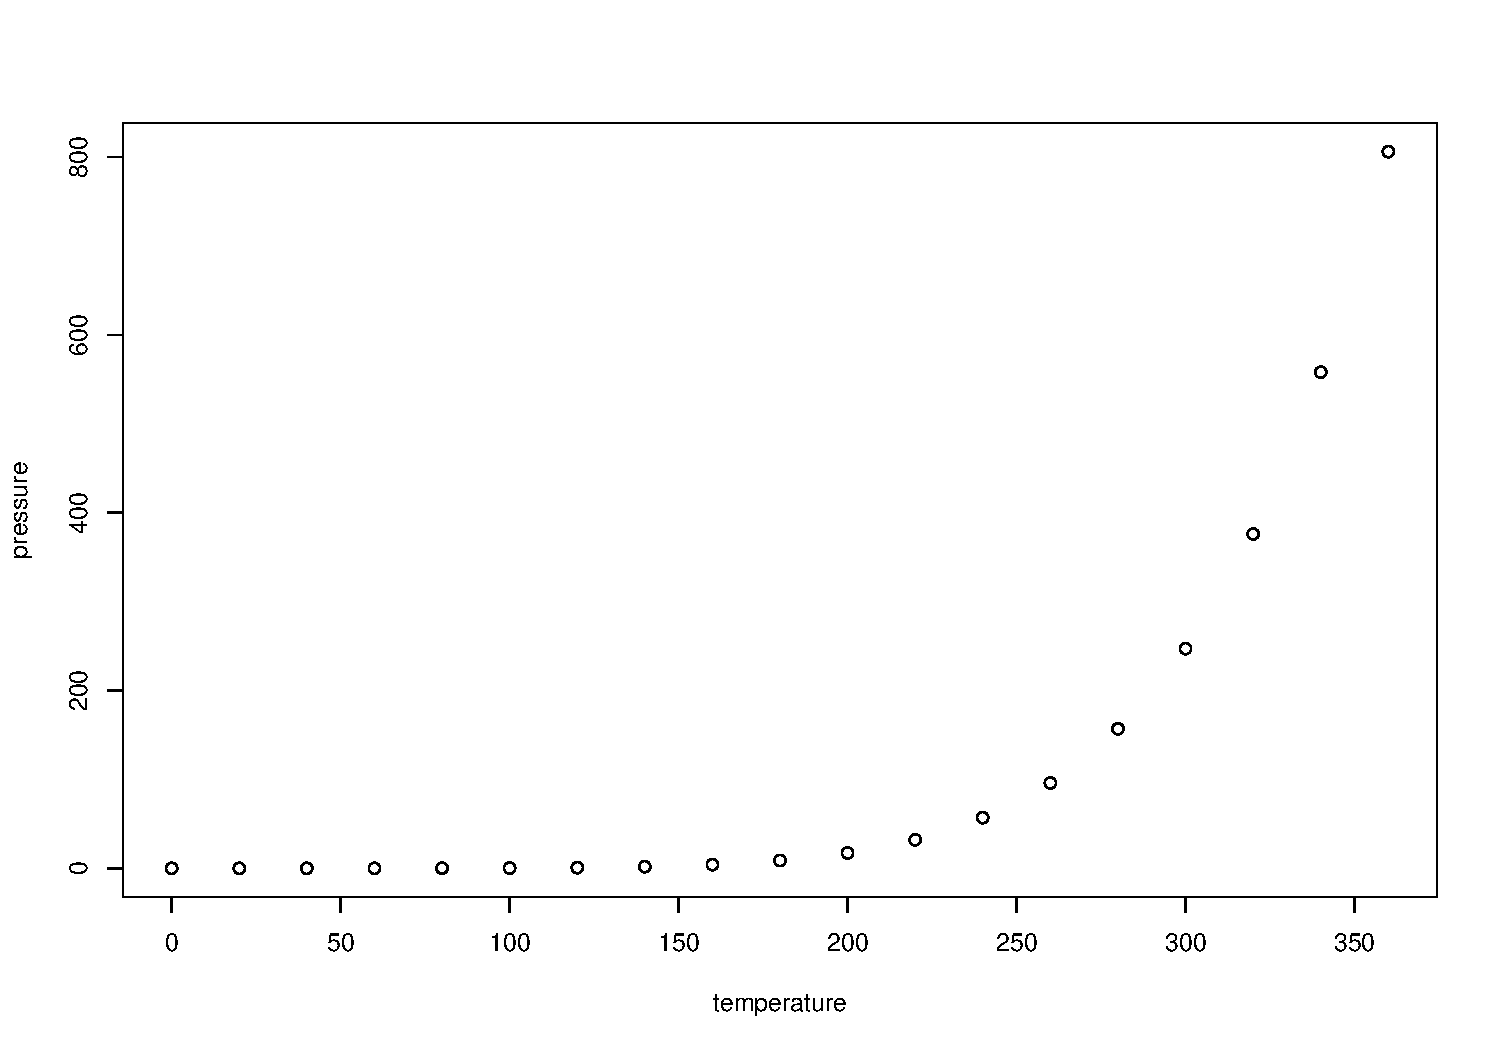
\includegraphics{Presentation_files/figure-beamer/unnamed-chunk-11-1.pdf}
- Is he willing to do what I want here?

\begin{itemize}
\item
  By which I mean automatically resizing the image at hand
\item
  He doesnt, not even now?
\end{itemize}
\end{frame}

\begin{frame}{Two column layout}
\protect\hypertarget{two-column-layout}{}
\footnotesize

\begin{columns}[T]
\begin{column}{0.48\textwidth}
\begin{figure}
\includegraphics[height=4cm]{Figures/Intro/Enrolment_over_time-1} \caption{Illustration of higher education system ideal types}\label{fig:unnamed-chunk-12}
\end{figure}
\end{column}

\begin{column}{0.48\textwidth}
\begin{itemize}[<+->]
\tightlist
\item
  Eat eggs
\item
  Drink coffee

  \begin{itemize}[<+->]
  \tightlist
  \item
    Have at it
  \end{itemize}
\end{itemize}
\end{column}
\end{columns}
\end{frame}

\begin{frame}{Final Test}
\protect\hypertarget{final-test}{}
Blocks

\begin{alertblock}{Theses}
1. The world is round \newline
2. It goes around
\end{alertblock}
\end{frame}

\begin{frame}[allowframebreaks]{Referenzen}
\protect\hypertarget{referenzen}{}
\hypertarget{refs}{}
\begin{CSLReferences}{1}{0}
\leavevmode\hypertarget{ref-Ansell.2008b}{}%
Ansell, Ben W. 2008. {``{University Challenges: Explaining Institutional
Change in Higher Education}.''} \emph{World Politics} 60 (2): 189--230.
\url{https://doi.org/10.1353/wp.0.0009}.

\leavevmode\hypertarget{ref-Ansell.2013}{}%
Ansell, Ben W., and Jane Gingrich. 2013. {``{A Tale of Two Trilemmas:
Varieties of Higher Education and the Service Economy}.''} In \emph{{The
Political Economy of the Service Transition}}, edited by Anne Wren,
195--226. Oxford: {Oxford University Press}.

\leavevmode\hypertarget{ref-garritzmann2016}{}%
Garritzmann, Julian L. 2016. \emph{{The Political Economy of Higher
Education Finance: The Politics of Tuition Fees and Subsidies in OECD
Countries, 1945-2015}}. Basingstoke: Palgrave Macmillan.
\url{https://doi.org/10.1007/978-3-319-29913-6}.

\leavevmode\hypertarget{ref-Gerring.2007}{}%
Gerring, John. 2007. \emph{{Case Study Research. Principles and
Practices}}. Cambridge: {Cambridge University Press}.

\leavevmode\hypertarget{ref-Hall.2001}{}%
Hall, Peter A., and David Soskice. 2001. {``Introduction.''} In
\emph{{Varieties of Capitalism. The Institutional Foundations of
Comparative Advantages}}, edited by Peter A. Hall and David Soskice,
1--68. Oxford: {Oxford University Press}.

\leavevmode\hypertarget{ref-Hall.1996}{}%
Hall, Peter A., and Taylor, Rosemary C. R. 1996. {``Political Science
and the Three New Institutionalisms.''} \emph{Political Studies} 44 (5):
936--57.

\leavevmode\hypertarget{ref-Mahoney.2010b}{}%
Mahoney, James, and Kathleen Thelen. 2010. {``{A Theory of Gradual
Institutional Change}.''} In \emph{{Explaining Institutional Change.
Ambiguity, Agency, and Power}}, edited by James Mahoney and Kathleen
Thelen, 1--37. Cambridge: {Cambridge University Press}.

\leavevmode\hypertarget{ref-Pierson.1993}{}%
Pierson, Paul. 1993. {``{When Effect Becomes Cause: Policy Feedback and
Political Change}.''} \emph{World Politics} 45 (4): 595--628.
\url{https://doi.org/10.2307/2950710}.

\leavevmode\hypertarget{ref-Streeck.2005}{}%
Streeck, W., and K. A. Thelen. 2005. \emph{{Beyond Continuity:
Institutional Change In Advanced Political Economies}}. {Oxford
University Press}.

\leavevmode\hypertarget{ref-Thelen.2004}{}%
Thelen, Kathleen. 2004. \emph{{How Institutions Evolve: The Political
Economy of Skills in Germany, Britain, the United States, and Japan}}.
Cambridge: {Cambridge University Press}.

\end{CSLReferences}
\end{frame}

\end{document}
